\subsection{Perceptual Losses for Real-Time Style Transfer and Super-Resolution}
\label{seq:johnson}
\textit{Perceptual Losses for Real-Time Style Transfer and Super-Resolution} is a paper written by Johnson et al. \cite{Johnson:1}. They take a new approach to solve the optimization problem proposed by Gatys et al \cite{Gatys:1}. Instead of doing a forward and backward pass through the pretrained VGG-network to solve every step of the optimization problem, which is computationally expensive, Johnson et al train an \textit{image transformation network} to approximate solutions to the optimization problem. The loss function for this network is based on the pretrained VGG-network, the \textit{loss network}. The feature maps which were discussed in Section \ref{sec:vgg} are used to train the image transformation network on high-level features, which in turn the define the \textit{perceptual loss functions}. This model just has to do one forward-pass to style an image, thus being much faster to style an image than the method of Gatys et al \cite{Gatys:1}. On the other hand, it is costly to train the model, as it is trained on a large dataset of different images, and it is not so flexible as it is trained to style an image with a particular style.
\subsubsection{Image transformation network}
\label{sec:neuralnetwork}
Johnson et al define an image transformation network $f_W$ which consists of $5$ residual blocks using the following architecture:\newline\newline
\begin{figure}[!ht]
\begin{center}
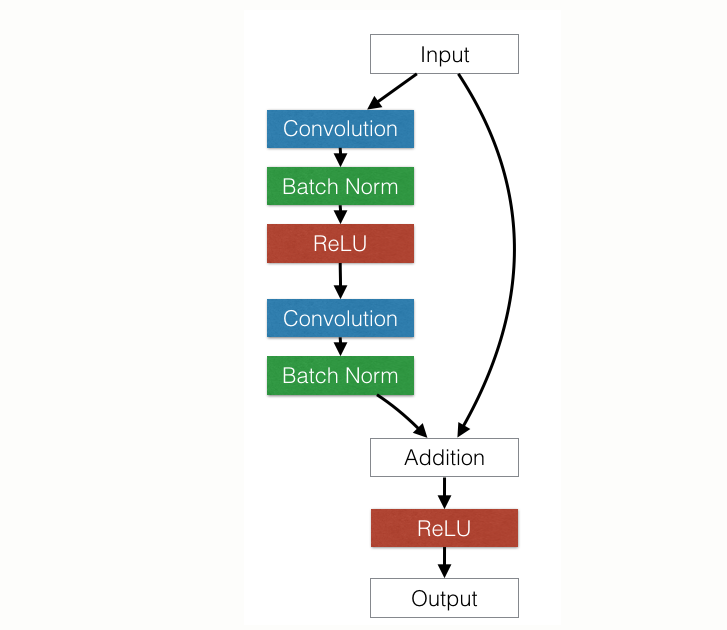
\includegraphics[scale=0.30]{report/Background/images/residualblock.png}
\caption{A residual block which adds an input $x$ to $x'$, where $x'$ is the result after doing some convolution, batch-normalization, and ReLU - operations on $x$. Then the ReLU-operation is performed on $x+x'.$}
\label{fig:residual}
\end{center}
\end{figure}\newline
All the layers non-residual layers are followed up by spatial batch normalizations and ReLU operations, except of the output layer, which is followed up by a scaled $\tanh$ operation. This is to ensure that the transformed image has pixels in the range $[0, 255].$\newline\newline
The main function of the image transformation network is to take an input image $x$, and produce the styled image $\hat{y}=f_W(x).$ The perceptual loss functions in the loss network calculate the loss, which will be discussed in Section \ref{sec:loss}. The loss is propagated back the network using back-propagation, and stochastic gradient descent is used to update the weights $W$ of the network.
\subsubsection{Perceptual loss functions}
\label{sec:loss}
Johnson et al define a loss network $\phi$, which defines several loss function $l_1,l_2,\dots,\l_k$. These loss functions can be categorized as two loss functions, one as the \textit{feature reconstruction loss} $l_{feat}^\phi,$ which is described by Equation (\ref{eq:content_loss}), and the other as the \textit{style reconstruction loss} $l_{style}^\phi,$ which is described by Equation (\ref{eq:style_loss}). So $l_i\in\{l_{feat}^\phi,l_{style}^\phi\}.$ When the image $\hat{y}$ has been produced by the image transformation network, a perceptual loss function calculates a scalar value $l_i(\hat{y}, y_i),$ where $y_i$ is a target image, either the content image or the style image. This loss is based on how equal the higher-dimensional feature maps of $\hat{y}$ and $y_i$ are, not $\hat{y}$ and $y_i$ themselves. These feature maps are extracted from the pre-trained loss network $\phi.$
\subsubsection{Architecture}
Johnson et al designed the following architecture, where they combine their fully-connected deep convolutional image transformation network $f_W$ with the pre-trained VGG loss network $\phi:$\newline
\begin{figure}[!ht]
\begin{center}
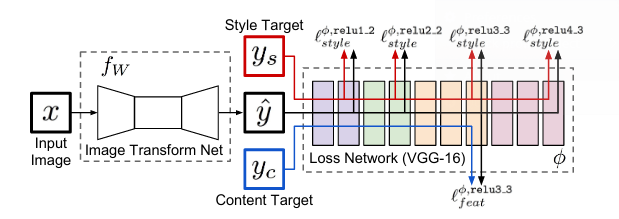
\includegraphics[scale=0.50]{report/Background/images/architecture.png}
\caption{The image transformation network $f_W$ transforms the image $x$ into $\hat{y}=f_W(x).$ After that, $\hat{y}$ is passed through the loss network $\phi$ to extract high-dimensional features. These features are compared with the features of $y_s$, the style target, and $y_c$, the content target.}
\label{fig:architecture}
\end{center}
\end{figure}\newline\newline
The image transformation network is trained with stochastic gradient descent, and the goal is to minimize
\begin{equation}
    W^*=\arg\min_W{\boldsymbol{E}_{x,\{y_i\}}\left[\sum_{i=1}{\lambda_il_i(f_W(x),y_i)}\right]}
\end{equation}
which is a weighed combination of the perceptual loss functions $l_i$.
\subsubsection{Instance normalization}
\label{sec:instance_normalization}
Instance normalization is a normalization method in used to train a model effectively. Although Johnson et al do not use instance normalization when they train their model, it is still worth to examine this normalization method, as it can be used to speed up the optimization of the image transformation network. Instance normalization was first introduced by Ulyanov et al in the paper \textit{Instance Normalization: The Missing Ingredient for Fast Stylization} \cite{Ulyanov:1}.\newline\newline
Before discussing instance normalization, let's look at Batch normalization. Batch normalization normalizes all the data across the batch and spatial locations. This normalization helps the network to converge faster, as the activations in the network converge towards unit Gaussian distribution. This prevents the \textit{vanishing gradient problem}, which means that the gradient of the loss function converges to $0$, making the model harder to train. The data $x_i$ is normalized in the following manner:
\begin{equation}
    x\leftarrow\frac{x-\mu_i}{\sqrt{\sigma_i+\epsilon}}
\end{equation}
where
\begin{equation}
\mu_i=\frac{1}{HWT}\sum_{t=1}^T\sum_{l=1}^W\sum_{m=1}^H{x_{tilm}}
\end{equation}
and
\begin{equation}
\sigma_i^2=\frac{1}{HWT}\sum_{t=1}^T\sum_{l=1}^W\sum_{m=1}^H{(x_{tilm}-mu_i)^2}
\end{equation}
Here $T$ is the number of batches. The downside with batch normalization is that it adds noise to the model, since it normalizes across the whole batch, so one instance depends on the neighbouring instances.\newline\newline
Instance normalization, however, normalizes each batch independently:
\begin{equation}
\mu_i=\frac{1}{HW}\sum_{l=1}^W\sum_{m=1}^H{x_{ilm}}
\end{equation}
and
\begin{equation}
\sigma_i^2=\frac{1}{HW}\sum_{l=1}^W\sum_{m=1}^H{(x_{ilm}-mu_i)^2}
\end{equation}
Here the model does not get extra noise, since the normalization is only happening across spatial locations. The calculation of instance normalization for a $x_i$ is $O(WH),$ while for batch normalization it is $O(TWH),$ where $O$ is Big $O$. This makes instance normalization both faster to compute, and the results get better because the noise is reduced.